\documentclass[10pt,conference,compsocconf]{IEEEtran}

\usepackage{hyperref}
\usepackage{graphicx}	% For figure environment
\usepackage{subfigure}
\usepackage{titling} % Customizing the title section
\usepackage{dblfloatfix}    % To enable figures at the bottom of page
\usepackage{kantlipsum}     % for random text
\usepackage{todonotes}

\begin{document}
\pretitle{\begin{center}\Huge\bfseries} % Article title formatting
\posttitle{\end{center}} % Article title closing formatting
\title{Road Segmentation challenge}

\author{
	% Your name
	\textsc{Niccol\`{o} Sacchi, Valentin Nigolian \& Theo Deprelle}
	\normalsize{} \\
	% Your supervisors
	\textsc{Group:}
	\normalsize{RoadSegmentationFault}\\
	% Your institution
	\normalsize \'{E}cole polytechnique f\'{e}d\'{e}rale de Lausanne
}

\maketitle

\begin{abstract}
  The goal of this project is to segment satellite images in order to discriminate the roads from the background. Several approaches have been tried in the past, most of them required a lot of preprocessing and did not gained great performances. Invented in the late 20th century, the convolutional neural networks (CNNs) only recently were successfully applied to images classification and segmentation problems and performed considerably better than other techniques.
  The models we propose in this project consist of two neural networks whose input can be an image of any size and the output is the respective mask of roads. Both the models make use of on-the-fly data augmentation, dropout layers and LeakyReLU or ReLU activation functions to reduce overfitting and improve the training. We will also show that, according to our tests, our models outperform the considered baselines.
\end{abstract}

\section{Introduction}
The segmentation problem can be defined as the problem of assigning a class label to a set of pixels so to classify part(s) of an image.
The goal of this project is to segment the roads in satellite images so to extract the mask of the roads. The metric used to evaluate the prediction of the roads is the F1 score that combines the precision, i.e. the fraction of correctly predicted roads among all the predicted roads, and the recall, i.e. the fraction of correctly predicted roads among all the true roads. The formula of the F1 score is the following:
$$F1=2\frac{pr}{p+r}$$ $$\textrm{where} \quad p=\frac{TP}{TP+FP} \textrm{,} \quad r=\frac{TP}{TP+FN}$$

Only in recent years, thanks the increase in computing performance and the possibility to exploit GPUs to parallelize computation, CNNs were able outperform most of the techniques in solving different tasks. The strengths of the CNNs derives from a hierarchy of filters which are learnt during the training phase. Thanks to these filters, the CNNs are capable of producing more and more complex features, i.e. high level representation of the input, as the image goes deeper in the network. However, a drawback of CNNs is the need of a large, fully-labeled dataset in order to extract the patterns proper of the objects that has to be recognized, otherwise the CNN would tend to overfit and just memorize the training dataset.
The following sections give an overview of the tried techniques focusing in particular on the two neural networks we implemented. Section~\ref{sec:data-analysis} gives an overview of the dataset, Section~\ref{sec:models-methods} proposes some approaches to the problem and explains the design of the two network used, Section~\ref{sec:results} shows and demonstrate the results reached with the explained models.

\section{Exploratory data analysis}
\label{sec:data-analysis}
We are given two sets of images acquired from GoogleMaps: (1) a train set composed by RGB images of size $400*400$ pixels and the respective ground-truth images, i.e. images of the same size where white pixels represent roads and black pixels represent the background, (2) a test set composed by RGB images of $608*608$ pixels whose ground-truth has to be predicted.
The aim of the project is to label the patches of size $16*16$ pixels. By taking a look at the train set and the respective ground-truth we could notice this task has its non-trivialities, e.g. the surface of the road is often covered by trees, shadows, buildings, railroads and/or cars, parking lots are sometimes marked as road and the roofs are of the same color of the roads. Those problems can be solved only if we consider also the neighborhood of each patch to correctly classify it. That task can be achieved only with proper with feature extraction, either manually, with complex and advanced techniques, or automatically by employing a CNN. Moreover, very few images have peculiar characteristic that differ from the rest of the images. Those are images of highways (3\% of the the dataset) and sea sides (2\% of the dataset). Some of these complications can be seen in Figure \ref{fig:corner-cases}.

\begin{figure}[h]
	\centering
	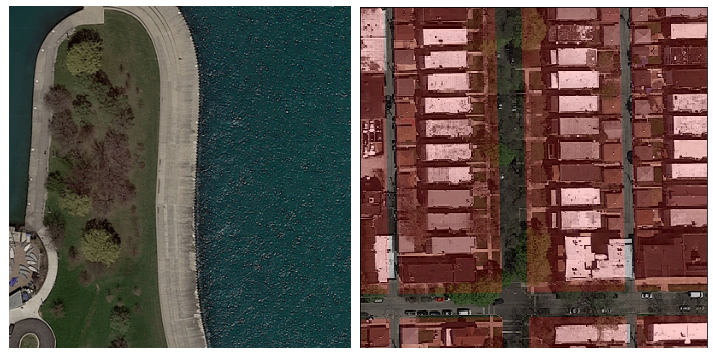
\includegraphics[width=\columnwidth]{img/corner_cases1.png}
	\vspace{-3mm}
	\caption{The left image is one of the very few sea sides images, the left image shows that roads may be covered by trees}
	\label{fig:corner-cases}
\end{figure}

\section{Models and Methods}
\label{sec:models-methods}
The first techniques we study involve feature extraction using interesting, still complex and not very efficient techniques that fails in more extreme cases, e.g. when there are object obstructing the view of the road or there is a change of brightness through different images. Such techniques involves for example computation of the gradient at each pixel (so to exploit the fact that roads have continuity in one direction, i.e. a gradient {\raise.17ex\hbox{$\scriptstyle\sim$}}0), the use of an edge detection algorithm to extract the boundaries of the objects and the use of vector graphics to represent images with geometrical primitives such as points, lines, curves, and shapes or polygons~\cite{HORMESE20161460}. Given the complexity of those solutions and poorness of the results when compared to the CNNs, we opt for the latter which are well know for the little preprocessing needed and great performances in solving these kind of tasks.
We start from three very simple baselines: (1) a model that predicts all as road (notice that, since the metric chosen is the F1 score computed on the road predictions, a model that predicts all as background would have higher accuracy but an F1 score of zero), (2-3) we consider each $16*16$ image patch as an input and for each one of them we produce 6 simple features extracted from the mean and the standard deviation of each RGB channel within the patch. We use the obtained dataset to train a logistic regression and a random forest. The F1 scores of these three baselines is shown in Figure \ref{fig:baselines}. As expected, this analysis shows that those methods fails in this complex task if more advanced features extraction is not in place.
Therefore, we study solutions based on CNNs and we find two main approaches: (1) design a CNN which segment the input image and outputs directly the mask for the roads~\cite{lis2016}, (2) reduce the segmentation problem to a classification problem, i.e. build a CNN that receives as input a single patch, possibly with a bigger context (neighborhood of that patch), and labels that patch as either road or background~\cite{dario2016}. We opt for the first choice as it requires almost no preprocessing. In particular, we implement two types of CNN models, a more traditional one and ... \todo{brief description of Théo model}. The two models, which are explained in the two following sub-sections, are accompanied by slightly different pre-processing and post-processing, e.g. data augmentation has been performed differently. Both the models can take as input an image of any size and output the respective mask of roads. To achieve such networks we do not use any dense layer which would require an input of fixed size. 

\begin{figure}[tbp]
	\centering
	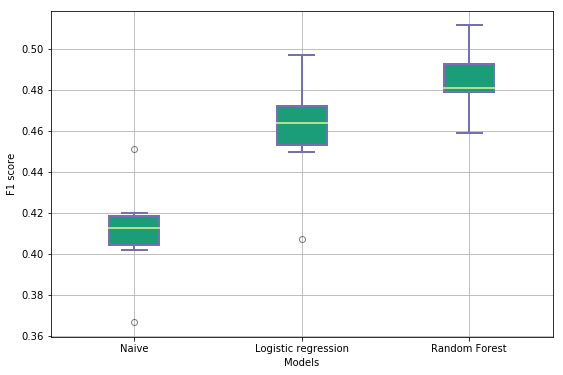
\includegraphics[width=0.8\columnwidth]{img/boxplots_naive.png}
	\caption{Distribution of the F1 scores computed on a 6-fold cross validation on the three considered baselines.}
	\vspace{-3mm}
	\label{fig:baselines}
\end{figure}

\subsection{Traditional CNN model}
\begin{figure}[tbp]
	\centering
	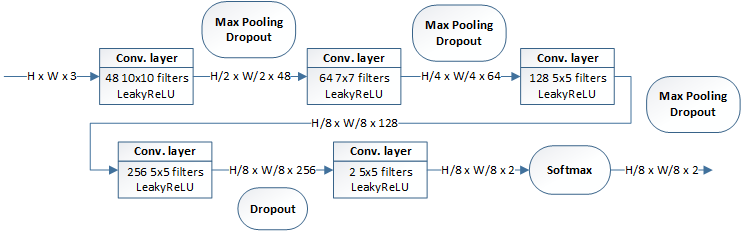
\includegraphics[width=\columnwidth]{img/cnnModel.png}
	\caption{Scheme of the CNN model which obtained an F1 score of XXX }
	\vspace{-3mm}
	\label{fig:cnn-model}
\end{figure}
\begin{figure}[tbp]
	\centering
	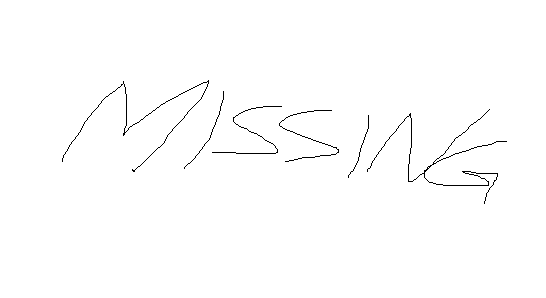
\includegraphics[width=0.8\columnwidth]{img/missing.png}
	\caption{Activations of the first convolutional layer: with ReLU on the left and with Leaky ReLU on the right. As can be noticed the number of dead filter decreased sensibly meaning the model was learning more reasonable features.}
	\vspace{-3mm}
	\label{fig:dead-filters}
\end{figure}

We designed this CNN so that it reduces each side of the input image by a factor equal to the width of the patch we want to predict so to obtain an output mask of size $H/n*W/n$ where $n$ is the width of the patch. In particular, we observed better results when predicting patches of size $8*8$. The structure of our CNN is depicted in Figure \ref{fig:cnn-model}. Since we experienced problems of GPU memory filling (when using a NVIDIA GeForce GTX 960), we could only adopt convolutional layers of higher number of filters in deeper layers, i.e. after reducing the size of the input image. In this way, the first layers have bigger inputs and less filters while the last layers have smaller inputs but can have more filters \footnote{The output of a convolutional layer, when strides is $1*1$ and padding is used (which is our case), is $H * W * \#filters$ where $H*W$ is the size of the input.}.

The most common activation function used after convolutional layer is the ReLU activation. However, since we have experienced the problem of dead filters \footnote{Dead filters are filters that always output zero for any input. This may happen when, during training, the weights are updated in such a way that the neuron will never activate on any input again which lead to a gradient of zero and no update of the weights.}, we have switched to the Leaky ReLU, i.e. a variant of the ReLU which has a small positive gradient for negative inputs:
$$f(x)=max(\alpha x, x)$$
Where $\alpha$ is the slope for negative inputs and is usually a small value ${\raise.17ex\hbox{$\scriptstyle\sim$}}0.01$.
This choice solved the problem of dead filters as can be seen in Figure \ref{fig:dead-filters}.

We used $k$ max pooling layers with a pool size of $2*2$ where $2\textsuperscript{k}$ is the size of the patch we wanted to predict, e.g. to predict $8*8$ patch-wise we adopted 3 max pooling layers so to reduce the size of the input image by a factor of 8 on each side. Note that increasing the strides of the convolutional layer would lead to the same size reduction but we opted for max pooling so to automatically select the highest activations.

Moreover, after each max pooling layer we added a dropout layer, i.e. a regularization technique used to prevent overfitting by randomly setting to 0 a fraction of the input during the training phase. We have set the dropping rate for all the dropout layers to $0.25$.

\subsubsection*{Data augmentation}
 This model is accompanied by on-the-fly batches of generation. In particular, the batches are generated by applying rotation and/or mirroring to the each image. While each image of the batch is mirrored with a probability of $0.5$ we decided to not rotate each image by a random degree since most of the images, both in the test set and train set, have vertical and horizontal roads and we wanted our model to master the recognition of those roads. Rotation is done in the following way: an image of the batch is rotated by any degree with a probability of $0.2$ while is rotated by $90^\circ*k$ where $k=1,2,3,4$ with a probability of $0.8$. Figure \ref{fig:data-augmentation} shows an examples of data augmentation applied on an image. This data augmentation proved to be effective and our model learnt not only to recognize horizontal and vertical roads but also diagonal roads.
\begin{figure}[tbp]
	\centering
	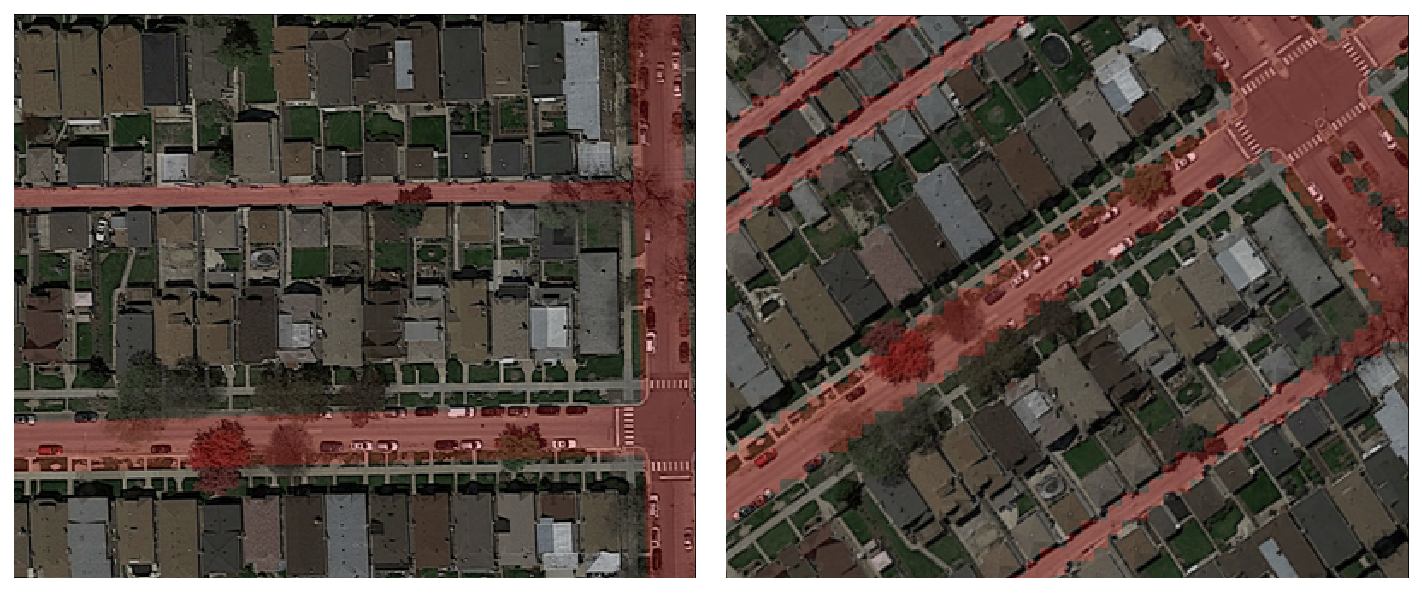
\includegraphics[width=0.8\columnwidth]{img/data_augmentation2.png}
	\caption{The left image is the original image. The right image is an example of augmentation of that image. After rotating the image, the points outside the boundaries are filled by reflecting the image so to always obtain an image of the same size ($400*400$).}
	\vspace{-3mm}
	\label{fig:data-augmentation}
\end{figure}

\subsubsection*{Post-processing}
Once the model have been trained, its the predictions can be further improved in order to increase the F1 score. However, even if roads have some intuitive properties, e.g. starting from a road you can always reach the border the image, it is not trivial to improve a predicted mask of roads such that those properties are fulfilled. Therefore, we opted for two easier solutions that proved to increase the F1 score sensibly.
\begin{itemize}
	\item We compute on the predictions of the training images the optimal threshold, i.e. if the probability of a patch is beyond that threshold then is labeled as road. This step is done with a grid search and by retrieving the threshold which corresponds to the maximum F1 score. This estimated optimal threshold will be used on the predictions of the test set to label each patch.
	\item To obtain the predictions of a test image, we mirror it and/or rotate it by $90^\circ*k$ where $k=1,2,3,4$ so to obtain 8 different predictions. Those predictions are then averaged to obtain the final mask of roads.
\end{itemize}

%~\cite{schwab00,wavelab,gentleman05}
%\begin{figure}[tbp]
%  \centering
%  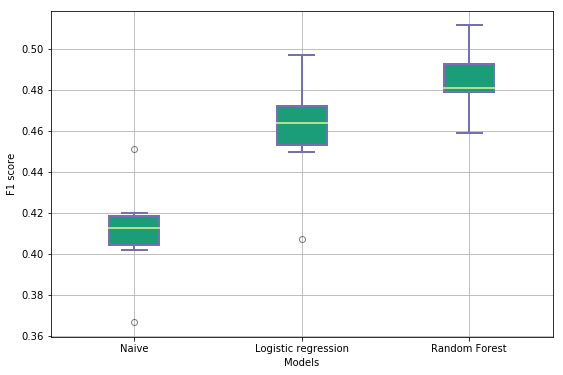
\includegraphics[width=\columnwidth]{img/boxplots_naive.png}
%  \caption{Signal compression and denoising using the Fourier basis.}
%  \vspace{-3mm}
%  \label{fig:denoise-fourier}
%\end{figure}
%
%\begin{enumerate}
%\item
%\end{enumerate}
%
%~\ref{tab:fourier-wavelet}.
%\begin{table*}[htbp]
%  \centering
%  \begin{tabular}[c]{|l||l|l|l|}
%    \hline
%    Basis&Support&Suitable signals&Unsuitable signals\\
%    \hline
%    Fourier&global&sine like&localized\\
%    wavelet&local&localized&sine like\\
%    \hline
%  \end{tabular}
%  \caption{Characteristics of Fourier and wavelet basis.}
%  \label{tab:fourier-wavelet}
%\end{table*}
%
%\footnote{For those who are
%  particularly interested, other common structures can be found at
%  \url{http://en.wikipedia.org/wiki/README} and
%  \url{http://www.gnu.org/software/womb/gnits/}.}.
%
%\texttt{.jpg} or
%
%\begin{equation}
%  \label{eq:linear}
%  y = mx + c
%\end{equation}
%(Equation~(\ref{eq:linear})).

\subsection{U-Net architecture}
The second model we have tried is the based on the U-Net architecture. This network was made to be used for medical image segmentation. Since our problem is close to what this network was made UNet was an ideal candidate.

U-Net network architecture is illustrated in \ref{fig:unet}. It consists of a down-sampling path (left side) and an up-sampling path (right side). Both share the architecture of a traditional CNN and consist of the repeated application of two 3x3 convolutions each followed by a Rectified Linear Unit (ReLU). However, while the down-sampling path contains 2x2 max pooling operations with stride 2, that reduce the dimension of the input, the up-sampling path up-convolutional layer \todo{is this sentence correct?} that increase the size of the input back to the size of the input image. Moreover, we are using four skip connections that performs a concatenation with the input of the maxpooling and the output of the up-convolution.

\begin{figure}[h]
  \centering
  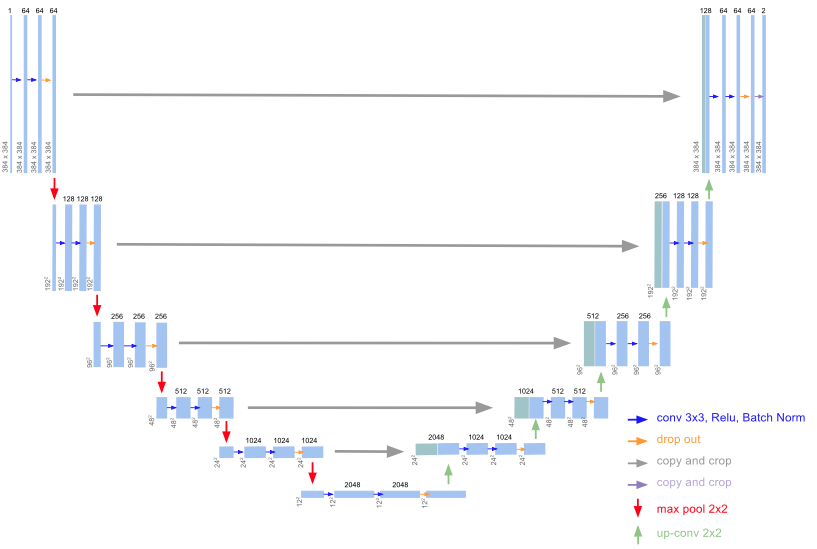
\includegraphics[width=0.95\columnwidth]{img/unet.png}
  \caption{UNet architecture}
  \label{fig:unet}
\end{figure}

We added to the existing architecture a batch normalization layer after every ReLU layers, a dropout layer before every max pooling and a fifth maxpooling operation.

The energy function is computed by a pixel-wise soft-max $S$ over the final feature map combined with the cross entropy loss function $E$.

\begin{equation}
	S(x) = \frac{exp(a_1(x))}{exp(a_1(x))+exp(a_0(x))}
\end{equation}

\begin{equation}
	E = \sum\limits_{x \in \Omega} w(x).log(S(x))
\end{equation}

Where $a_k(x)$ denotes the activation in feature channel $k$ at the pixel position $x$ of the image $\Omega$.

\subsubsection*{Data augmentation}

\begin{figure}[h]
 \centering
 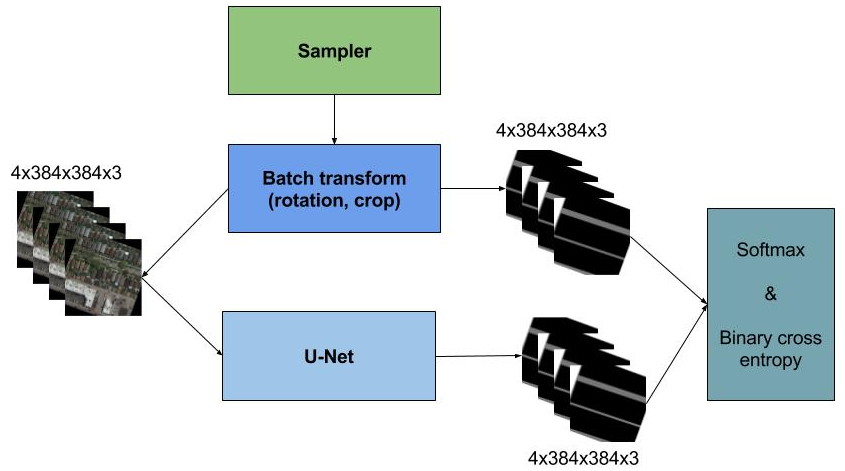
\includegraphics[width=0.7\columnwidth]{img/dataaug.png}
 \caption{Training step diagram.}
 \vspace{-3mm}
 \label{fig:denoise-fourier}
\end{figure}

We trained the network  batches of 4 images. Each image of the batch is a randomly selected patch of size $384*384$ from the original image. Using this method our result were good but it appears that diagonal roads were not detected correctly. This was because the majority of the images of the training set did not had diagonal lines. To correct this problem we randomly rotate the image after every training step. This allows us to have a better diagonal roads detection since the train set now included roads of different orientations, see Figure \ref{fig:diagonal}. However, rotating an image may leave some pixels outside the boundaries. We decided to label those pixels in the ground-truth with a different class, i.e. class 2 (ignore part). Those labels allowed us to ignore the respective pixel in the computation of the loss, which was properly modified, so that they have no impact on the training process.

\begin{figure}[h]
 \centering
 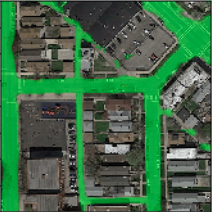
\includegraphics[width=0.35\columnwidth]{img/diagonals.png}
 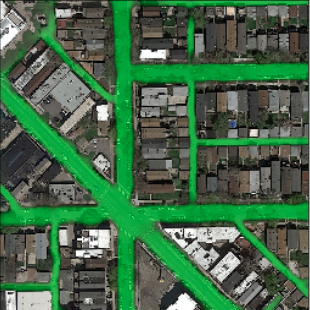
\includegraphics[width=0.35\columnwidth]{img/diagonals_corrected.png}
 \caption{On the left we can see that the diagonals are not detected well. On the contrary, on the right, when we are randomly rotating the images all the diagonals are well detected}
 \vspace{-3mm}
 \label{fig:diagonal}
\end{figure}

\section{Results}
\label{sec:results}
\subsection{Traditional CNN}
	The traditional CNN was trained for XXX epochs, each consisting of XXX batches of 4 images, on a NVIDIA GeForce GTX graphics card with 2 GB of VRAM. 
	\todo{change this, we can say we don't use the cross validation but precision-recall method => add to figure 9 the line representing the traditional cnn}
	In order to compare different CNNs models we used 4-fold cross validation. Figure XX shows the estimated F1 scores of our main CNN models compared to the aforementioned three baselines and agrees with the F1 score obtained on Kaggle (XXX\%). Even without any preprocessing other than data augmentation our CNN outperformed the baselines and confirmed their superiority in solving this kind of tasks.
\subsection{U-Net}
	After 10000 iteration with a learning rate $\lambda = 10^{-3}$ we have obtained a accuracy of 93.35\% on the test set where the labels are unknown.
	To compare different techniques we used the Precision Recall method (PR) which focuses on the relevance of the prediction on the labels of a test set. To compute the PR values we split the training dataset into two subsets, one used for training and one used to compute the PR curve. The latter is computed by gradually increasing the threshold (used to establish, given its probability, if a pixel is a road) to compute different PR values. In this way, we obtain the graph in Figure \ref{fig:pr}.
	\begin{figure}[h]
		\centering
		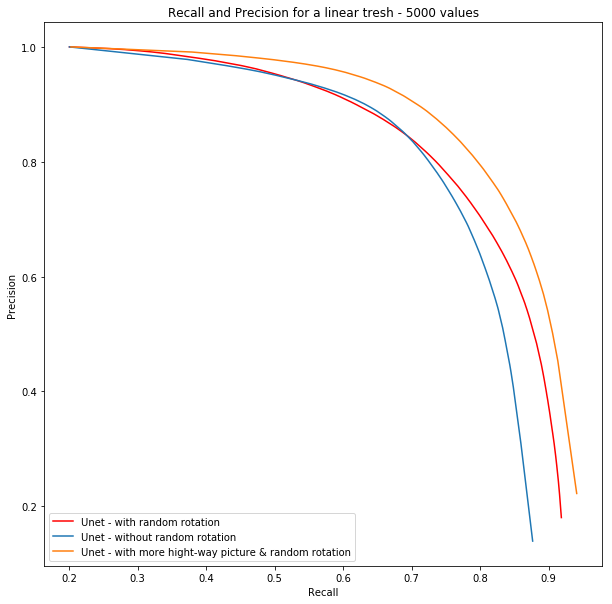
\includegraphics[width=0.8\columnwidth]{img/pr_curve.png}
		\caption{Precision and recall evolution regarding our different methods}
		\label{fig:pr}
	\end{figure}
	\todo{explain what those curves have to be interpreted}
	With U-Net we can see the evolution with the different approaches. The random rotation and the enhancement of the highway images (we repeated the few highway images of the train set in order to improve the prediction of wide roads) are improving the performance of the model.

\section{Conclusion}
\label{sec:conclusion}
Both models proved to be versatile and effective in predicting correctly. However, our traditional CNN model failed in recognizing narrow roads, especially when they were covered by shadows, those types of roads are indeed almost inexistent in the training set while present in many images of the test set. Moreover, the train and test datasets were mainly restricted to cities. To obtain a model that would efficiently work with a wider range of input images, e.g. images with snow, country images or on different meteorological conditions, we would require a bigger and diverse training set.

\bibliographystyle{IEEEtran}
\bibliography{groupRoadSegmentationFault-literature}

\end{document}
